\section{Технологический раздел}

\subsection{Выбор системы управления базами данных}

При выборе системы управления базами данных были выделены критерии:
\begin{enumerate}[label*=---]
	\item бесплатное и открытое программное обеспечение;
	\item поддержка процедурных расширений языка SQL;
	\item наличие личного опыта работы.
\end{enumerate}

\begin{table}[hbtp]
	\begin{center}
		\begin{flushleft}
			\captionsetup{justification=raggedright, singlelinecheck=false}
			\caption{\label{tab:bd}Сравнение систем управления базами данных}
		\end{flushleft}
		\begin{tabular}{|  p{0.20\textwidth} | p{0.23\textwidth} | p{0.25\textwidth}  |  p{0.18\textwidth}|} 
			\hline  Система управления базами данных & Бесплатное и открытое программное обеспечение & Поддержка процедурных расширений языка SQL  &  Наличие личного опыта работы \\ \hline
			PostgreSQL~\cite{postgres} &     + & + & + \\ \hline
			Oracle~\cite{oracleReal} &   -  &   + & -  \\ \hline
			MySQL~\cite{mysql} &  + &  - & - \\ \hline
		\end{tabular}
	\end{center}
\end{table}

Исходя из сравнения в таблице~\ref{tab:bd} в качестве системы управления базами данных в данной работе будет использоваться PostgreSQL.

\subsection{Архитектура приложения}

Для приложения была выбрана клиент-серверная архитектура. Доступ к серверной части будет осуществляться с помощью API~\cite{api}. Чтобы выполнять запросы к базе данных, будут применяться коннекторы, которые обеспечивают интерфейс взаимодействия через язык программирования. Приложение разделено на следующие компоненты: компонент доступа к данным, компонент бизнес-логики и компонент интерфейса. Верхнеуровневое разбиение на компоненты представлено на рисунке~\ref{img:upper}.
\begin{figure}[!h]
	\centering
	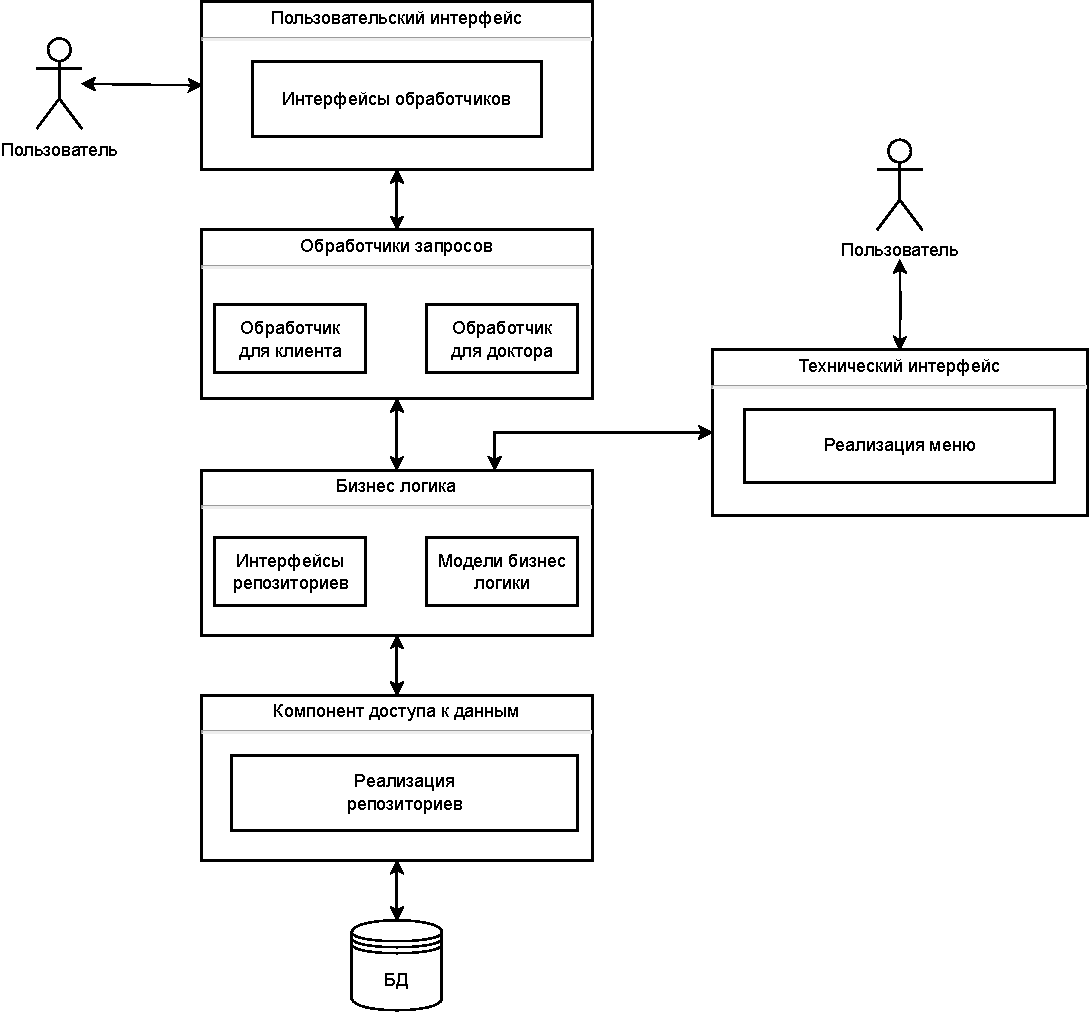
\includegraphics[width=\textwidth]{image/upper}
	\caption{Верхнеуровневое разбиение на компоненты}
	\label{img:upper}
\end{figure}

\newpage

\subsection{Средства реализации}

В рамках данной работы были выбраны следующие технологии.
\begin{enumerate}[label=\arabic*)]
	\item Язык программирования -- Golang~\cite{go}.
	\item Система управления базами данных -- PostgreSQL. 
	\item Для написания хранимых процедур базы данных будет использовано расширение языка SQL -- PL/pgSQL~\cite{pgSQL}.
	\item Для работы с СУБД была выбрана библиотека database/sql~\cite{go-sql}, предоставляющая универсальный интерфейс для реляционных баз данных, а также ее расширение -- библиотека sqlx~\cite{sqlx}.
	\item Фреймворк для реализации API -- gin~\cite{gin}.
	\item Для обечпечения безопасности паролей пользователей была использована хэш-функция bcrypt~\cite{bcrypt}. 
	\item Аутентификация была реализована на основе Bearer-токенов~\cite{bearer}.
	\item Для автоматизации развертывания и изолирования приложения была выбрана платформа Docker~\cite{docker}. 
	\item Технический интерфейс -- консоль. 
\end{enumerate}

\newpage
\subsection{Детали реализации}

\subsubsection{Создание таблиц}

В конструкторском разделе было спроектировано 6 таблиц в базе данных с ограничениями и первичными ключами. В листинге~\ref{tables} представлен соответствующий код создания таблиц.  

\begin{code} 
	\captionof{listing}{Скрипт создания таблиц}
	\label{tables}
	\inputminted
	[
	frame=single,
	framerule=0.5pt,
	framesep=10pt,
	fontsize=\small,
	tabsize=4,
	linenos,
	numbersep=5pt,
	xleftmargin=10pt,
	]
	{text}
	{code/tables.sql}
\end{code}

\subsubsection{Создание ролей на уровне базы данных}

В конструкторской части были выделены 4 роли на уровне базы данных: гость, клиент, доктор и администратор. Создание ролей и выделение им прав, в соответствии с ролевой моделью, представлены в листинге~\ref{role}. 

\begin{code} 
	\captionof{listing}{Скрипт создания ролевой модели базы данных}
	\label{role}
	\inputminted
	[
	frame=single,
	framerule=0.5pt,
	framesep=10pt,
	fontsize=\small,
	tabsize=4,
	linenos,
	numbersep=5pt,
	xleftmargin=10pt,
	]
	{text}
	{code/roles.sql}
\end{code}

\subsubsection{Создание триггера}

В конструкторской части был разработан триггер для проверки валидности новой записи с помощью расширения PL/pgSQL, используемого в системе управления базами данных PostgreSQL. Код триггера и соответствующей функции представлен в листинге~\ref{func}. 

\begin{code} 
	\captionof{listing}{Триггер проверки валидности новой записи}
	\label{func}
	\inputminted
	[
	frame=single,
	framerule=0.5pt,
	framesep=10pt,
	fontsize=\small,
	tabsize=4,
	linenos,
	numbersep=5pt,
	xleftmargin=10pt,
	]
	{text}
	{code/func.sql}
\end{code}

\subsection{Тестирование}

Для тестирования проекта были реализованы модульные тесты для компонента доступа к данным и для компонента бизнес-логики. Также написаны интеграционные тесты для связи двух компонентов. Каждый тест выполняется в отдельном Docker контейнере, до теста запускается скрипт создания таблиц и в случае необходимости база данных заполняется тестовыми данными. 

Для автоматизации тестирования, проведения исследования и развертывания использовался инструмент Gitlab CI/CD~\cite{ci}. Был создан сценарий, состоящий из четырех стадий. 
\begin{enumerate}[label=\arabic*)]
	\item Pre. Стадия состоит из статического анализа кода и инициализации модулей. 
	\item Test. Стадия содержит модульное тестирование компонента бизнес-логики и компонента доступа к данным, а также интеграционное тестирования.
	\item Build. Состоит из сборки серверной части приложения и технического интерфейса.
	\item Research. Содержит исследование, описанное в следующем разделе.
\end{enumerate}
Задания, входящие в каждую из стадий приведены на рисунке~\ref{stages}. 
\begin{figure}[!h]
	\centering
	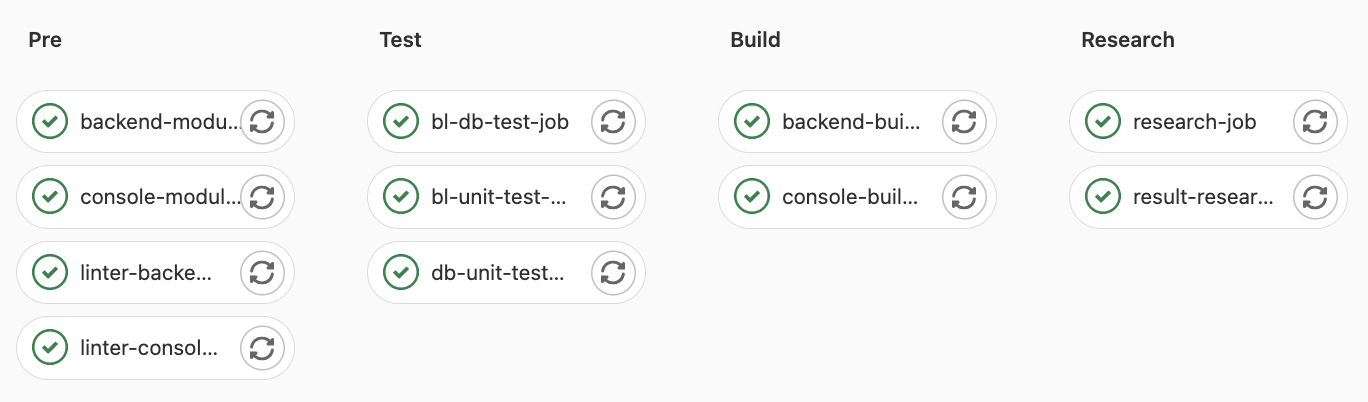
\includegraphics[width=\textwidth]{image/stages}
	\caption{Стадии сборочной линии}
	\label{stages}
\end{figure}

Серверная часть приложения и технический интерфейс не связаны между собой, но имеют общие стадии. На рисунке~\ref{needs} изображена зависимости между заданиями сборочной линии. 
\begin{figure}[!h]
	\centering
	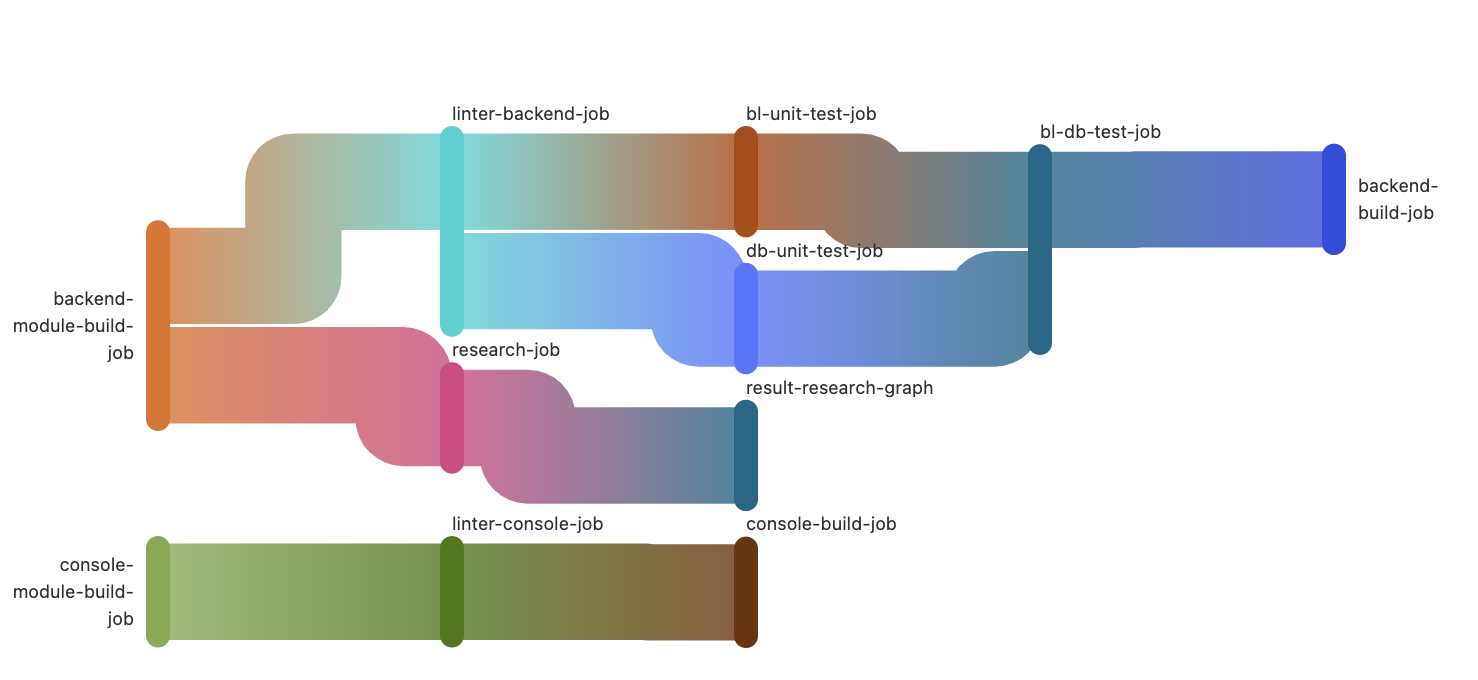
\includegraphics[width=\textwidth]{image/needs}
	\caption{Зависимости между заданиями}
	\label{needs}
\end{figure}


\subsection*{Вывод}
В данном разделе была описана архитектура приложения, средства и детали его реализации. Приведена сборочная линии для тестирования и развертывания приложения, а также проведения исследования с помощью инструмента Gitlab CI/CD.

